\documentclass[tikz,border=10pt]{standalone}
% No extra TikZ libraries needed
\begin{document}
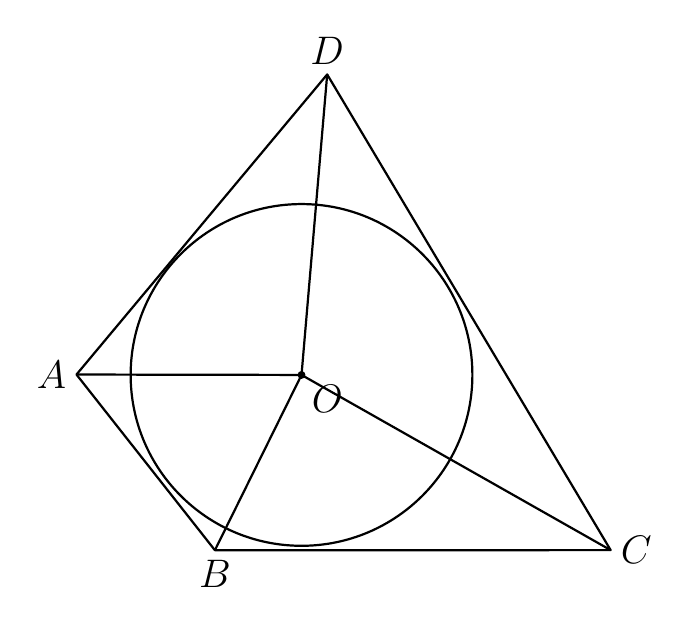
\begin{tikzpicture}[line join=round, line width=0.8pt, font=\fontsize{15.5}{18.6}\selectfont]
  % Vertices and centre (scale s = 0.013491 cm/px, y flipped); CV-derived, unchanged
  \coordinate (D) at (-0.208,3.019);
  \coordinate (A) at (-3.392,-0.792);
  \coordinate (B) at (-1.634,-3.023);
  \coordinate (C) at (3.392,-3.022);
  \coordinate (O) at (-0.534,-0.797);

  % Circle centred at O, radius 2.17 cm
  \draw (O) circle[radius=2.17];

  % Quadrilateral sides D-A-B-C
  \draw (D) -- (A) -- (B) -- (C) -- cycle;

  % Segments from O to each vertex
  \draw (O) -- (A);
  \draw (O) -- (B);
  \draw (O) -- (C);
  \draw (O) -- (D);

  % Centre dot
  \fill (O) circle[radius=0.05];

  % Vertex labels
  \node[above] at (D) {$D$};
  \node[left] at (A) {$A$};
  % B label centred directly below vertex B
  \node[below] at (B) {$B$};
  \node[right] at (C) {$C$};
  \node[below right] at (O) {$O$};
\end{tikzpicture}
\end{document}